\chapter{电容式离子电流检测电路实验台架}
\section{实验台架}
本实验台架由发动机,发动机支架,发动机附加和其他测试设备组成。其台架系统示意图如\ref{fig:platformintro}图所示。
\begin{figure}[!h]
	\centering
	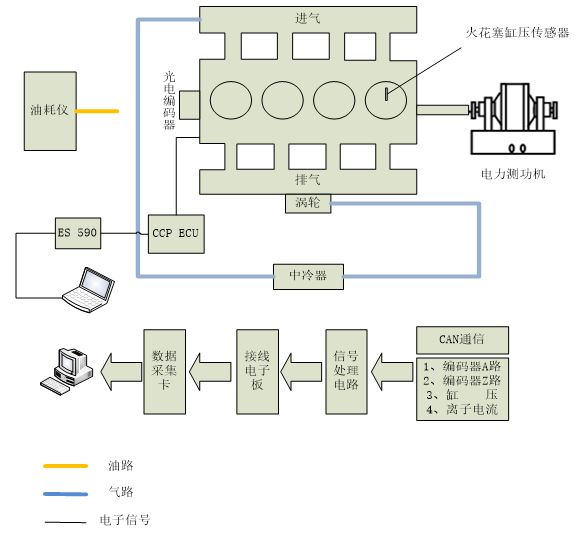
\includegraphics[width=0.85\textwidth]{thesis_figure/platformer_chapter/platformer_intro}
	\caption{台架系统示意图}
	\label{fig:platformintro}
\end{figure}
其中发动机是搭载于长安睿骋1.8T的涡轮增压多点进气道喷射发动机,电力测功机为南丰测功机,油耗仪为AVL油耗仪,通过Kistler火花塞式缸压传感器来测量缸压,用光电编码器
来同步信号并确定曲轴上止点位置。通过改造普通的点火线圈将二级线圈高压点和接地点接入离子电流采集电路中来采集离子电流信号。其实物图如图\ref{fig:platformintro_real}所示。
\begin{figure}[t]
	\centering
	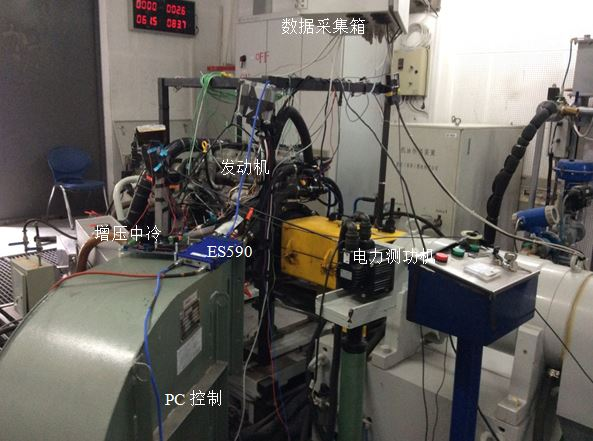
\includegraphics[width=0.8\textwidth]{thesis_figure/platformer_chapter/platformer_intro_real}
	\caption{台架系统实物图}
	\label{fig:platformintro_real}
\end{figure}
\subsection{发动机}
发动机为搭载于长安睿骋1.8T上的涡轮增压PFI发动机,其实物图如\ref{fig:ecu}所示,其具体参数如表\ref{tab:ice}所示。
其ECU为联合汽车电子有限公司提供的基于ME788控制系统的ECU,实物图如图\ref{fig:ice}所示。
\begin{figure}[!ht]
	\begin{minipage}[h]{0.5\linewidth}
		\centering
		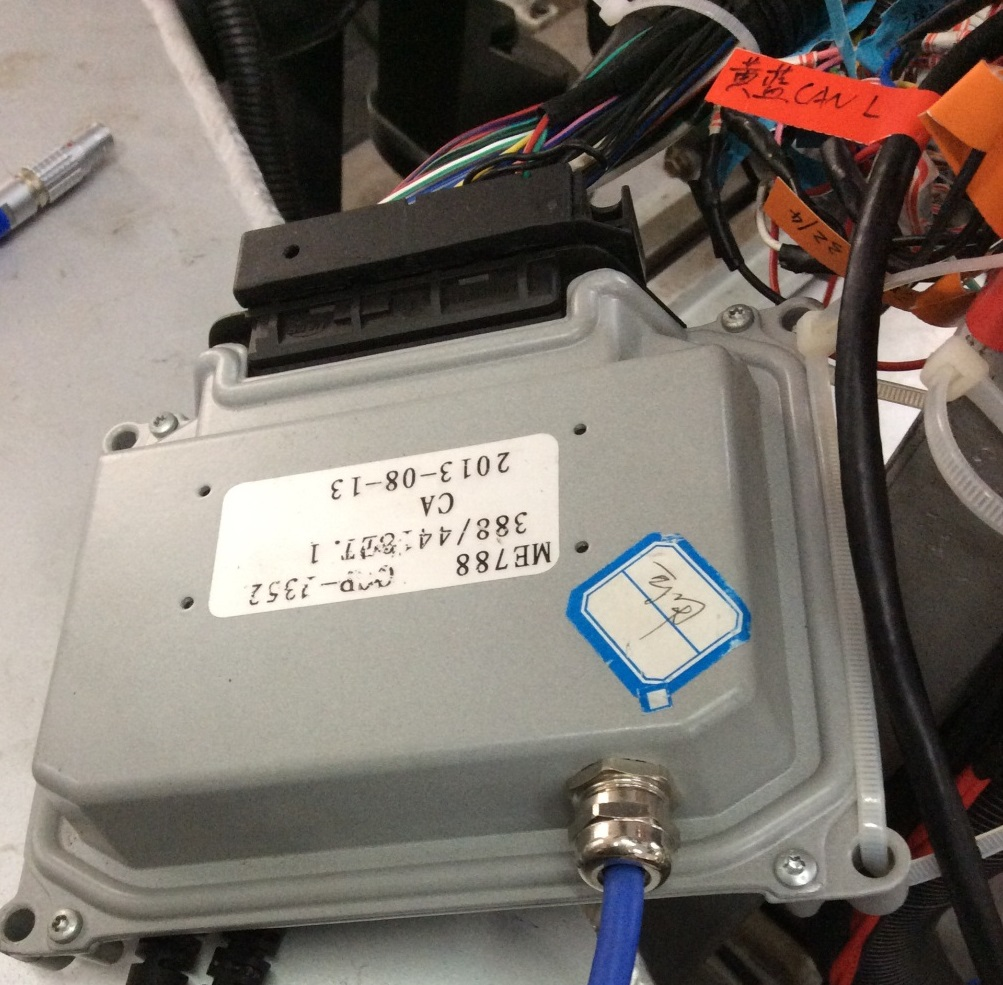
\includegraphics[width=0.8\textwidth]{thesis_figure/platformer_chapter/ecu}
		\caption{ECU实物图}
		\label{fig:ecu}
	\end{minipage}
	\begin{minipage}[h]{0.5\linewidth}
		\centering
		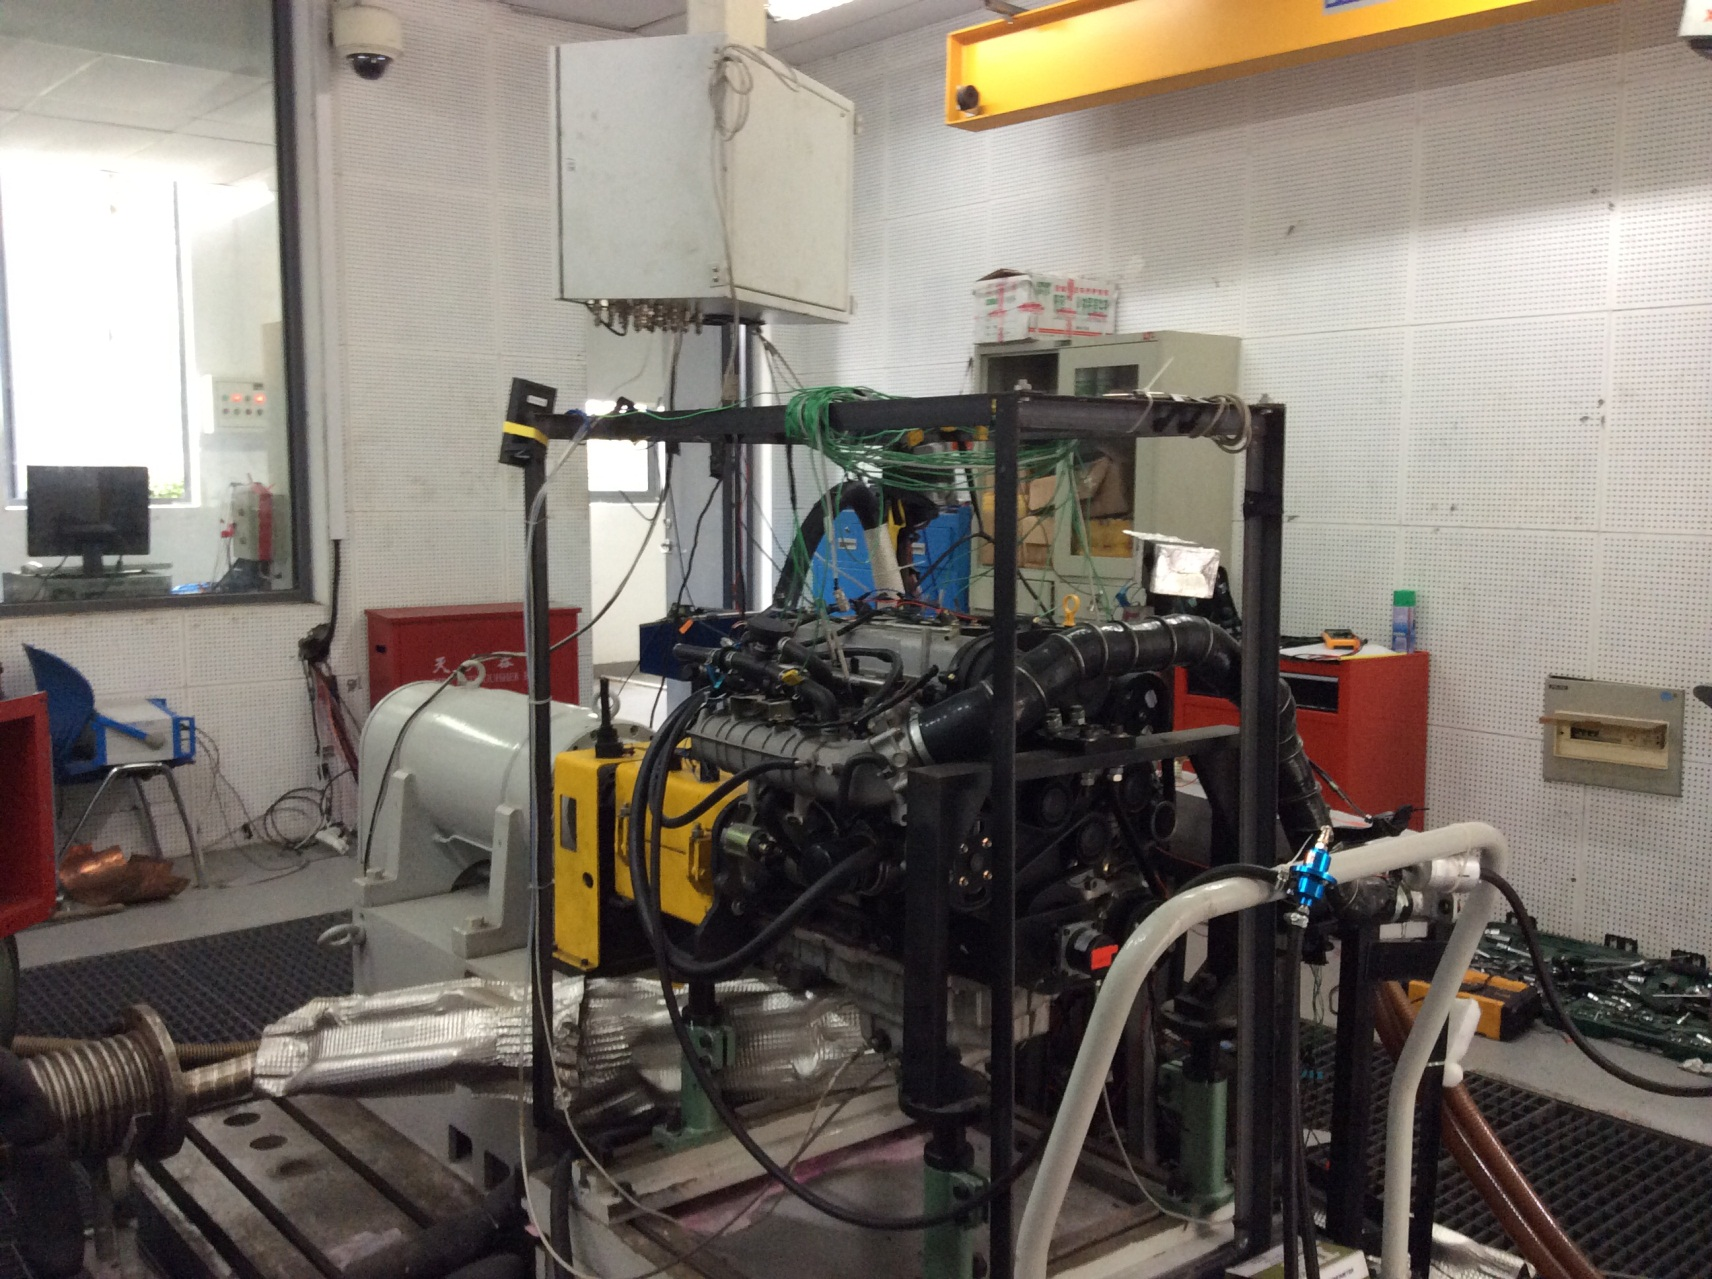
\includegraphics[width=\textwidth]{thesis_figure/platformer_chapter/ice}
		\caption{发动机实物图}
		\label{fig:ice}
	\end{minipage}
\end{figure}
\begin{table}[ht]
	\centering
	\caption{发动机具体参数}
	\label{tab:ice}
	\begin{tabular}{c|c}
		\hline
		发动机类型 & 4冲程PFI涡轮增压发动机 \\\hline
		排量(cc) & 1798 \\\hline
		最大功率(kW) & 130 \\\hline
		最大扭矩(Nm) & 230 \\\hline
		缸径(mm) & 86 \\\hline
		行程(mm) & 77.4 \\\hline
	\end{tabular}
\end{table}
\par 通过INCA等软件将该ECU的数据显示并保存出来,用MDA对保存的数据进行简单的数据分析。

\subsection{发动机支架}
发动机支架主要由发动机安装活动平台和可调螺旋支架两部分组成。该发动机安装活动平台由框架、耐磨导轨、高精度
定位装置、导向装置、锁紧机构、耐磨承重车轮及集污盘等组成,实物见图\ref{fig:hdpt}。该活动安装平台通过高精度定位销来保证
平台的横向和纵向距离,保证了固定在该活动平台上的发动机可以和测功机的飞轮衔接处的精度,同时提高了该活动平台的复用性,从而
有效地减少了发动机安装和调试所占用的时间。发动机支架由转接工装、ZJ系列可调支架、横梁等组成,可满足30至800KW发动机的支撑
要求。同时,此活动平台有很高的兼容性,对于多种发动机都适用,可以实现发动机的三位调整。
\begin{figure}[!h]
	\begin{minipage}[h]{0.5\linewidth}
		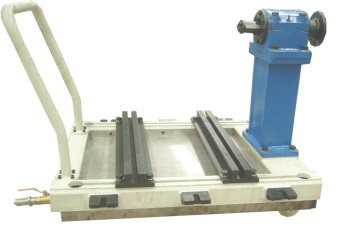
\includegraphics[width=0.8\textwidth]{thesis_figure/platformer_chapter/hdpt}
		\caption{发动机安装活动平台}
		\label{fig:hdpt}
	\end{minipage}%
	\begin{minipage}[h]{0.5\linewidth}
		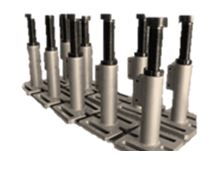
\includegraphics[width=0.8\textwidth]{thesis_figure/platformer_chapter/lxzj}
		\caption{可调螺旋支架}
		\label{fig:ktzj}
	\end{minipage}
\end{figure}
\par 可调螺旋支架由活动的减震杆和T型底座两部分组成,实物见图\ref{fig:ktzj}两个部分之间通过螺纹孔连接。T型底座可以在发动机安装活动平台的耐磨导轨上
沿小车纵向运动,通过两个螺栓可以固定其横向位置。减震杆采用较为柔软的金属制作而成,且通常在安装过程中在其上垫入一些金属片提高减震
效果。减震杆顶部有螺纹孔,方便发动机支架与之固定。
\begin{figure}[h]
	\centering
	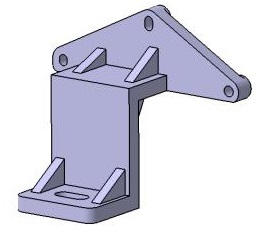
\includegraphics[width=0.3\textwidth]{thesis_figure/platformer_chapter/zj1}
	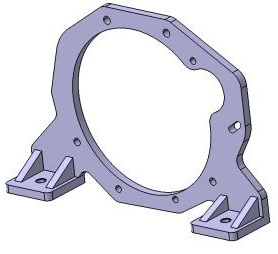
\includegraphics[width=0.3\textwidth]{thesis_figure/platformer_chapter/zj2}
	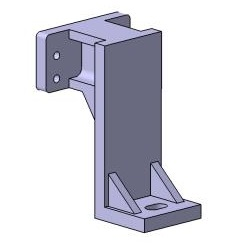
\includegraphics[width=0.3\textwidth]{thesis_figure/platformer_chapter/zj3}
	\caption{发动机支架部件图}
	\label{fig:zjbjt}
\end{figure}
\par 基于以上的两种基本结构,设计了改款发动机的支架结构。选择发动机气缸体上表面作为测量基准水平平面,选择飞轮端平面为基准垂直面,利用水平尺、直角尺和
游标卡尺等量具测量固定发动机的螺栓孔与基准面间的空间距离。使用CATIA三维机械设计软件搭建了发动机支架的三维模型,并将其装配到虚拟发动机模型上。
飞轮端支架采用龙门式结构,足够承受径向和轴系的交变载荷;通过焊接加强肋与安装固定销的方式,保证在正时链条端的两个支架结构紧凑,同时充分考虑扰度和
抗变形能力。经过反复测量并制作放样模型修正支架参数,完成支架设计。整体支架焊接采用拼接工艺,每个部件均使用销定位直角面,并加工卡槽阶梯面减少支架在焊
接后产生的形变。如图\ref{fig:zjbjt}所示。
\subsection{测功机}
交流电力测功机是目前市场上最先进的动力加载测试设备,其可兼顾各动力机械低俗及高速的加载测功实验,在性能、可靠性及维护难易程度等方面都有比较明显的优势。
本次实验采用的交流电力测功机系统来自凯迈(洛阳)机电有限公司,该测功机系统基于先进变频技术平台开发,其具有低惯性、高精度、高稳定性、结构简单、维护方
便、自成系列并适用于操作控制自动化等优点。如图\ref{fig:dlcgj}是测功机安装布线的示意图。
\begin{figure}[H]
	\centering
	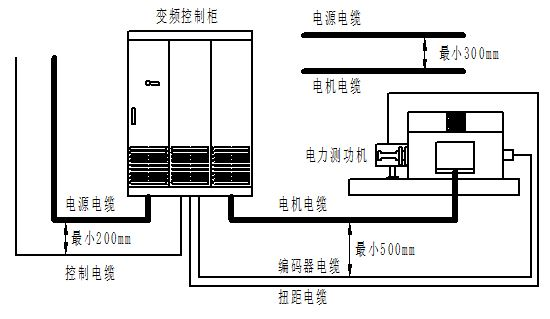
\includegraphics[width=0.5\textwidth]{thesis_figure/platformer_chapter/dlcgj}
	\caption{DCW系列交流电力测功机系统安装布线示意图}
	\label{fig:dlcgj}
\end{figure}
\par 该交流电力测功机主要由一台三相异步交流电机(含高精度转速编码器、精密扭矩法兰)、一套可四象限运行的交流调速柜、控制系统、采集系统组成。交流变频调速柜分为整流
单元和逆变单元两部分组成。整流单元的可控硅将用户输入的380V交流电转换为内部之流点,该直流电再逆变为电压及频率可变的交流电输出到三相异步电机。
\begin{figure}[H]
	\centering
	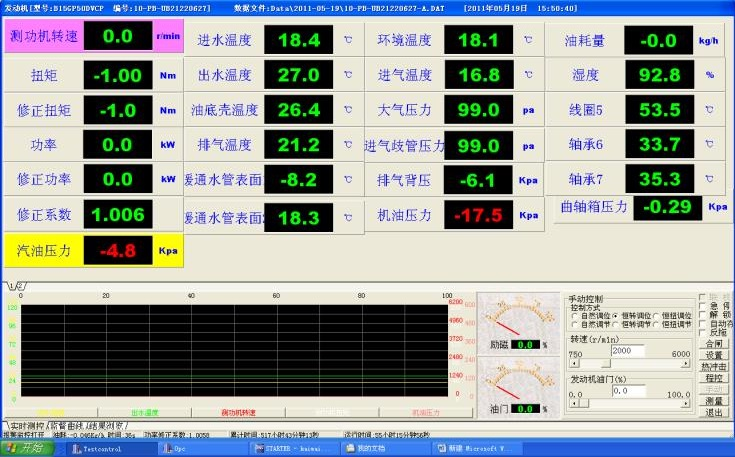
\includegraphics[width=0.8\textwidth]{thesis_figure/platformer_chapter/cgjkzjm}
	\caption{测功机控制界面}
	\label{fig:cgjkzjm}
\end{figure}

\begin{figure}[H]
	\centering
	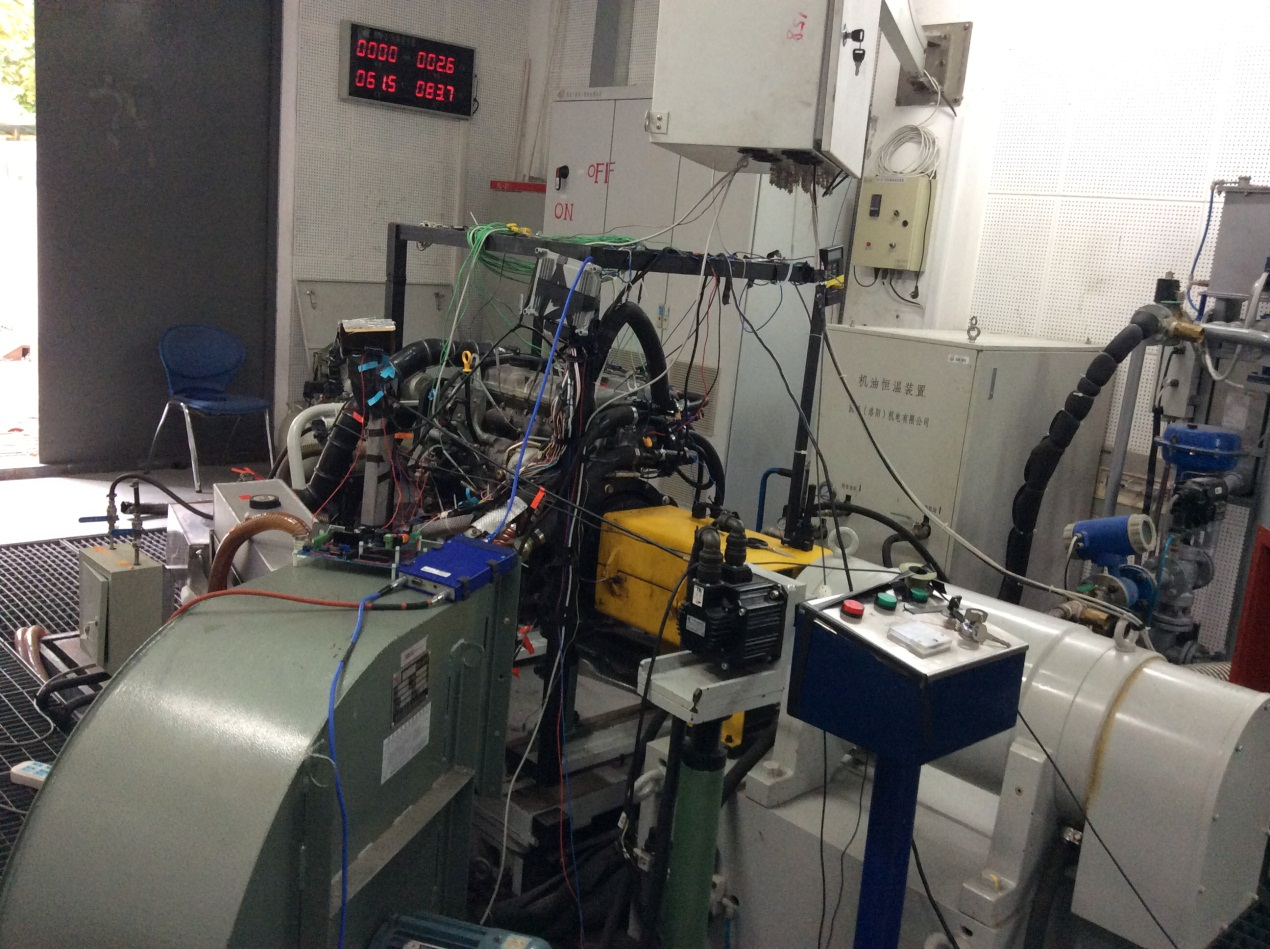
\includegraphics[width=0.65\textwidth]{thesis_figure/platformer_chapter/dlcgjswt}
	\caption{电力测功机实物图}
	\label{fig:dlcgjswt}
\end{figure}
\par 测功机的实物图如\ref{fig:dlcgjswt}所示,其具体参数如表\ref{tab:dlcgjjtcs}所示。在拖动状态时,通过调整交流电的频率及电压以改变转速,达到拖动负载的目的;在发电状态时,通过电机的四象限转换,将电机产生的交流电转变为直流电再经过整流单元转换
为符合上网要求的交流电,传到电网,以达到加载转矩的目的。测功机控制界面如图\ref{fig:cgjkzjm}所示,该界面实时显示台架试验过程中转速、水温、扭矩等状态参
数,并具有急停功能。
\begin{table}[H]
	\centering
	\caption{电力测功机具体参数}
	\label{tab:dlcgjjtcs}
	\begin{tabular}{ccc}
	\hline
	测量参数 & 测量范围 & 精度\\\hline
	转速 & $0\thicksim10000r/min$ &$\pm 1 r/min$ \\
	扭矩 & $0\thicksim500N\centerdot m$ &$\pm 0.4 \%FS$ \\
	燃油消耗 &$0\thicksim100Kg/h$ & $\pm 0.12\% FS$ \\
	环境温度 &$0\thicksim50^{\circ}C$ & $\pm 0.5\% FS$ \\
	环境湿度 &$0\thicksim100\%$ & $\pm 2\% RH$ \\
	冷却水进温 &$0\thicksim150^{\circ}C$ & $\pm 0.5^{\circ}C$ \\
	冷却水出温 &$0\thicksim150^{\circ}C$ & $\pm 0.5^{\circ}C$ \\
	机油温度 &$0\thicksim150^{\circ}C$ & $\pm 0.5^{\circ}C$ \\
	燃油温度 &$0\thicksim150^{\circ}C$ & $\pm 0.5^{\circ}C$ \\
	中冷前温度 &$0\thicksim150^{\circ}C$ & $\pm 0.5^{\circ}C$ \\
	中冷后温度 &$0\thicksim250^{\circ}C$ & $\pm 0.5^{\circ}C$ \\
	排气温度 &$0\thicksim150^{\circ}C$ & $\pm 0.5^{\circ}C$ \\
	机油压力 &$0\thicksim1000KPa$ & $\pm 0.5\%FS$ \\
	燃油压力 &$0\thicksim1000KPa$ & $\pm 0.5\%FS$ \\
	进水压力 &$0\thicksim600KPa$ & $\pm 0.5\%FS$ \\
	出水压力 &$0\thicksim600KPa$ & $\pm 0.5\%FS$ \\
	曲轴箱压力 &$-20\thicksim20KPa$ & $\pm 0.25\%FS$ \\
	排气背压 &$0\thicksim50KPa$ & $\pm 0.5\%FS$ \\
	中冷前压力 &$0\thicksim300KPa$ & $\pm 0.5\%FS$ \\
	中冷后压力 &$0\thicksim300KPa$ & $\pm 0.5\%FS$ \\
	大气压力 &$80\thicksim110KPa$ & $\pm 0.25\%FS$ \\\hline
	\end{tabular}
\end{table}
\subsection{发动机附件}
发动机附件包括增压中冷系统、冷却系统、进排气系统等。
\par \textbf{增压中冷系统}
\par 增压中冷系统由中冷器、进气、出气、进水、出水、增压压力温度传感器等部分组成,实物图如图\ref{fig:zyzlq}所示。
\begin{figure}[H]
	\centering
	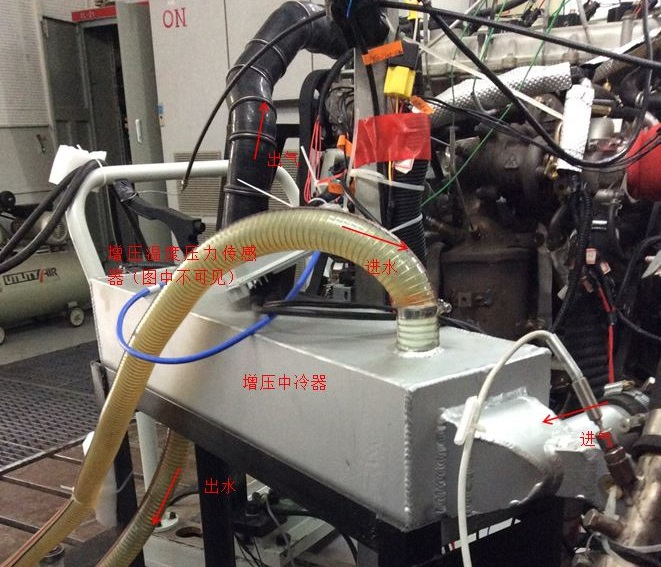
\includegraphics[width=0.7\textwidth]{thesis_figure/platformer_chapter/zyzlq}
	\caption{发动机增压中冷系统}
	\label{fig:zyzlq}
\end{figure}
\par \textbf{冷却系统}
\par 冷却系统分为水冷和风冷两部分,水冷由外接的冷却循环系统构成,如图\ref{fig:sllqxt}所示。风冷则主要是使用大功
率的风机吹排气管,实现快速降温,使温度在需要范围之内,如图\ref{fig:fllqxt}所示。
\begin{figure}[H]
	\centering
	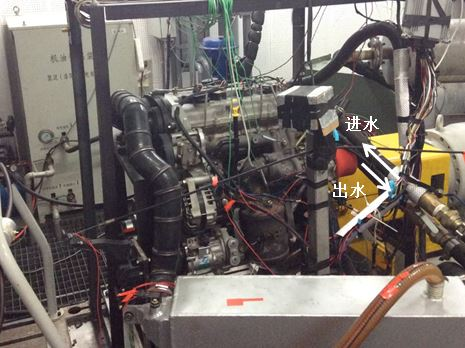
\includegraphics[width=0.7\textwidth]{thesis_figure/platformer_chapter/sllqxt}
	\caption{发动机外接水冷系统}
	\label{fig:sllqxt}
\end{figure}
\begin{figure}[H]
	\centering
	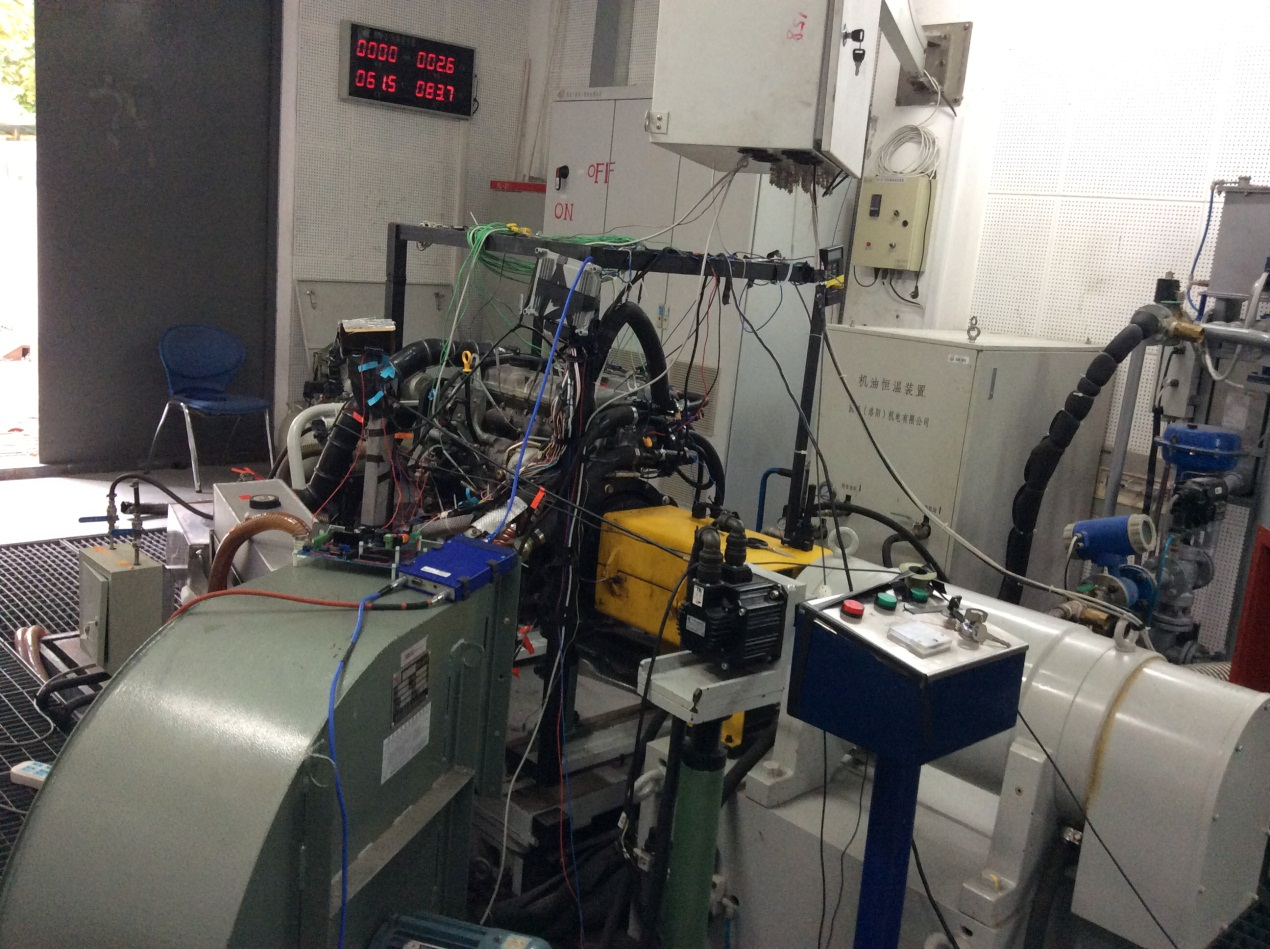
\includegraphics[width=0.7\textwidth]{thesis_figure/platformer_chapter/fllqxt}
	\caption{发动机外接风冷系统}
	\label{fig:fllqxt}
\end{figure}
\par \textbf{进排气系统}
\par 进气系统由自制空气滤清器和原机进气管组成,排气系统由原机排气歧管、排气管加上自制一段排气管通往实验室排气系统中,
其中,排气管上装有排气温度传感器,排气系统如图\ref{fig:jpqxt}所示。
\begin{figure}[H]
	\centering
	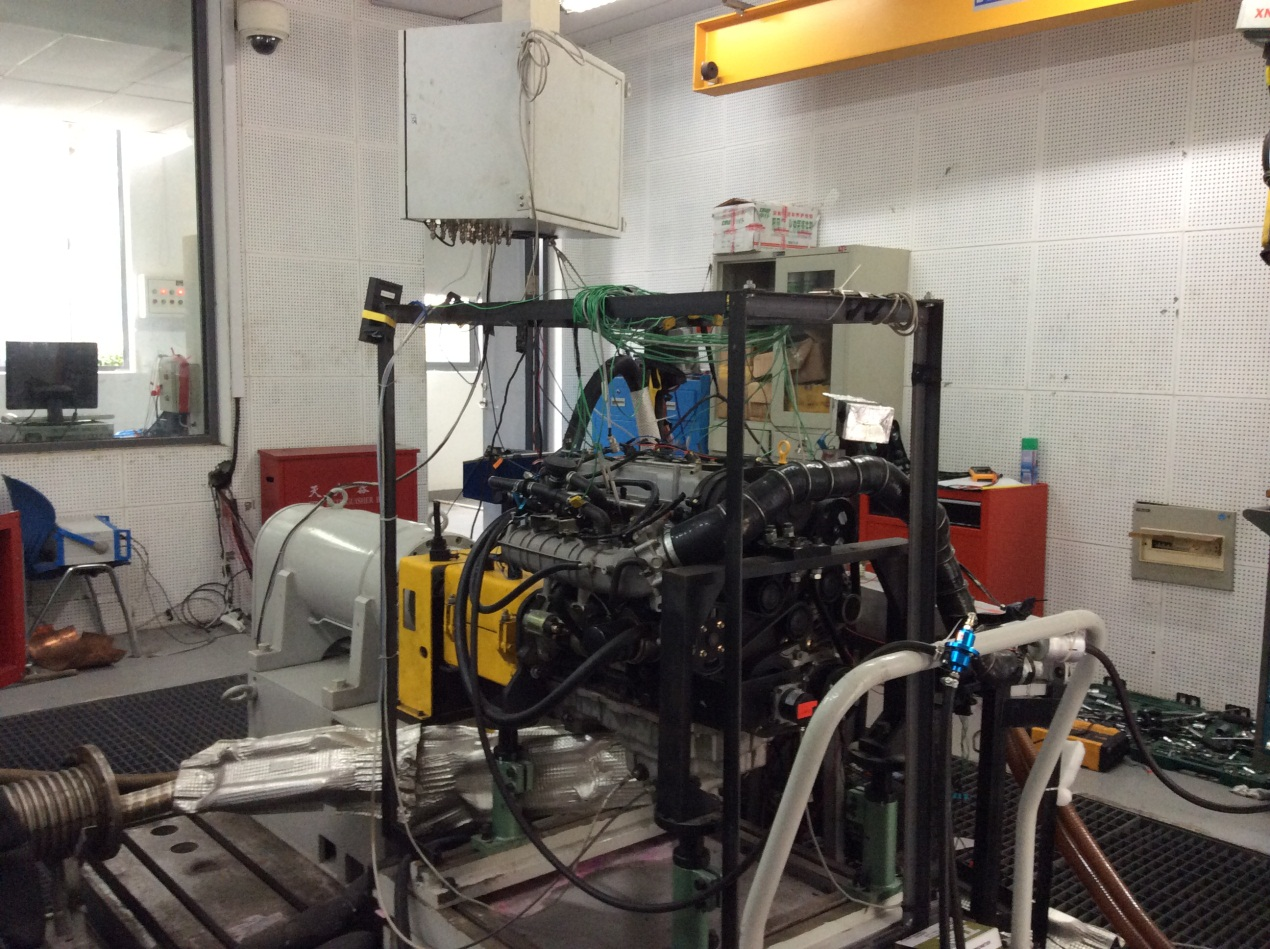
\includegraphics[width=0.7\textwidth]{thesis_figure/platformer_chapter/jpqxt}
	\caption{发动机进排气系统}
	\label{fig:jpqxt}
\end{figure}
\section{实验设备及器材}
\subsection{缸压传感器}
缸压传感器采用的是KISTLER 提供的6118B型火花塞缸压传感器,具有完整的3mm缸压传感器和可换电缆,无需另外打孔即可实
现缸压的测量。
\begin{table}[H]
	\caption{缸压传感器具体参数}
	\label{tab:gycgq}
	\centering
	\begin{tabular}{ccc}
	\hline
	物理量 & 单位& 数值 \\
	\hline
	重量 & g& 50\\
	压力范围 & bar & $0\thicksim 200$ \\
	标定区间(在200$^{\circ}C$) &bar & $0\thicksim 150$ \\
	过载 & bar & 250 \\
	灵敏度(200$^{\circ}C$) & pC/bar & $\thickapprox10$ \\
	固有频率 & kHz & $>100$ \\
	室温线性度 & \%FSO & $\leq \pm$ 0.5 \\
	加速的灵敏度(轴向和径向) & bar/g & $<0.005$ \\
	传感器工作温度范围 & $^{\circ}C$ & $-20\thicksim 350$ \\
	电缆工作温度范围 & $^{\circ}C$ & $-20 \thicksim 200$ \\
	灵敏度变化($200\pm 50^{\circ}C$)&\%& $\leq\pm 1$ \\
	短期飘移$\triangle p$ & bar & $\leq \pm 0.6$ \\
	$\triangle p_{min}$ & \% & $\leq \pm 3$ \\
	$\triangle p_{max}$ & \% & $\leq \pm 1.5$ \\
	20$^{\circ}C$时传感器绝缘阻抗 & $\Omega$ & $>1013$ \\
	200$^{\circ}C$时传感器绝缘阻抗 & $\Omega$ & $>1011$ \\
	火花塞阻抗(1000V,室温下) & $\Omega$& $>100$ \\
	绝缘强度 & kV& $<35$ \\
	传感器电容 & pF/m& 110\\
	\hline
	\end{tabular}
\end{table}
它装有世界上最小的压电式高温缸压传感器。安装时,前端与燃烧室内部平齐,固有频率高于100kHz。因此,也可用
于高速发动机和爆震控制测试。其实物图和技术参数见图\ref{fig:gycgq}和表\ref{tab:gycgq}。其还配备了装有数字式双
通道电荷放大器模块的信号调理平台,信号放大范围为$\pm 100\thicksim 10000$pc/V,通过将放大后的气缸压力信号传
给工控机采集卡记录缸内燃烧压力数据。
\par 这种电荷放大器可以用于实验室通过压电测力仪测量力和扭矩。通过负载作用在压电传感器上产生一个正比例变化的电荷。这
个电荷信号放大器转换成比例的输出电压。电荷放大器的实物图如图\ref{fig:gycgqdhfdq}所示。
\begin{figure}[ht]
	\begin{minipage}[H]{0.5\linewidth}
		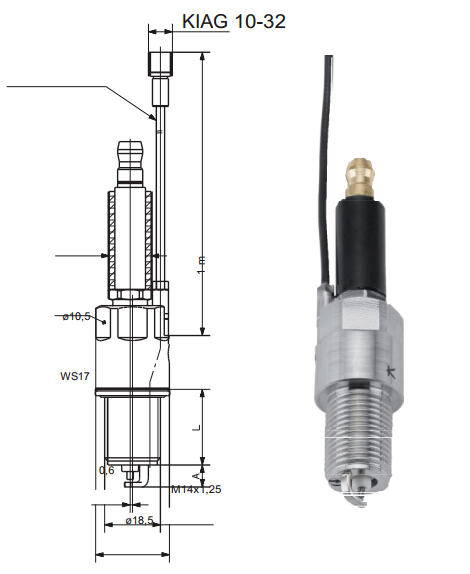
\includegraphics[width=0.8\textwidth]{thesis_figure/platformer_chapter/gycgq}
		\caption{火花塞式缸压传感器}
		\label{fig:gycgq}
	\end{minipage}
	\begin{minipage}[H]{0.5\linewidth}
		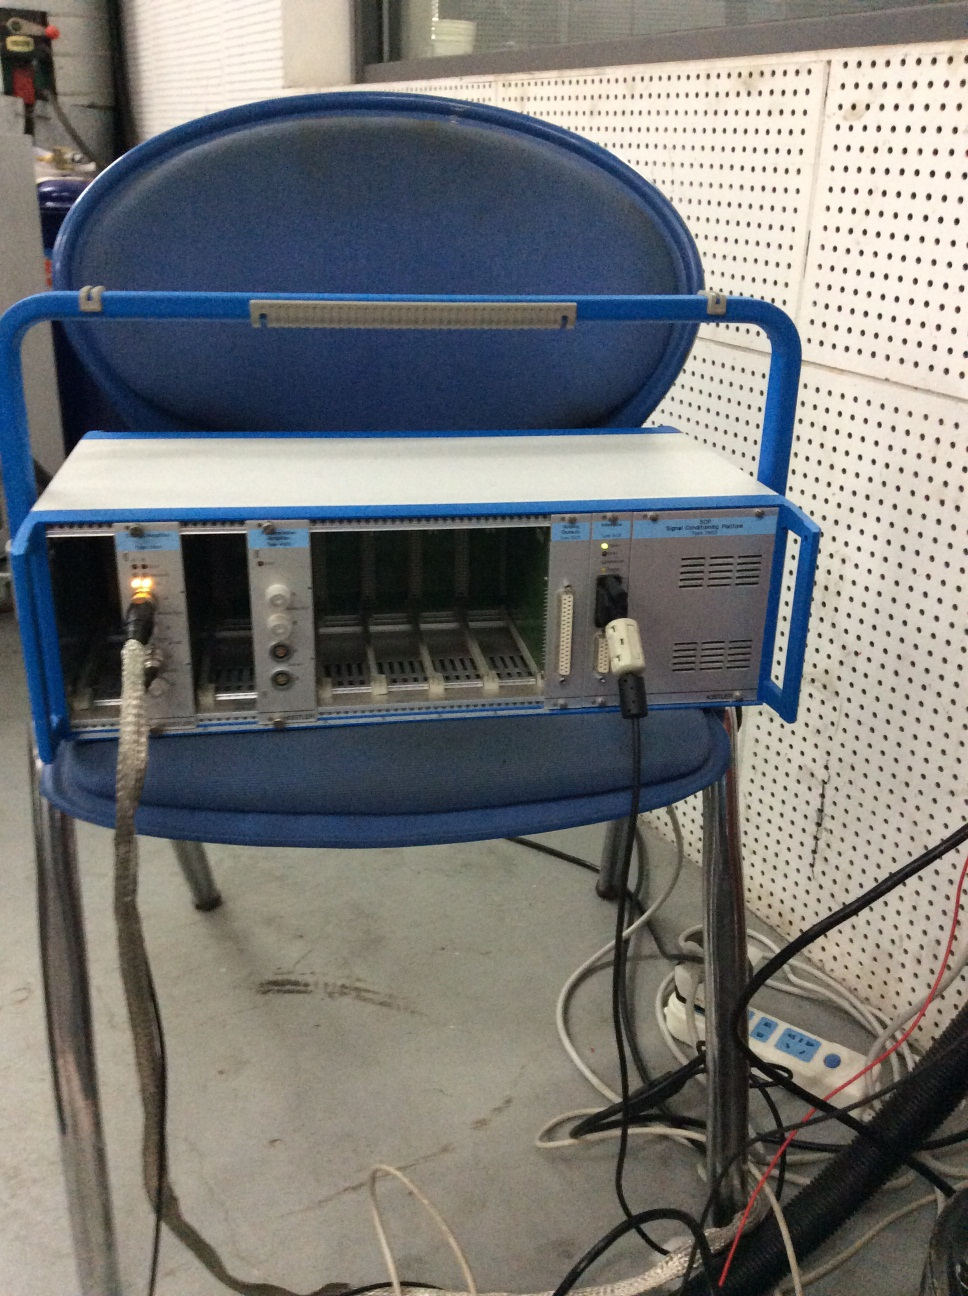
\includegraphics[width=0.8\textwidth]{thesis_figure/platformer_chapter/gycgqdhfdq}
		\caption{缸压传感器电荷放大器}
		\label{fig:gycgqdhfdq}
	\end{minipage}
\end{figure}
\subsection{光电编码器}
发动机正时链条侧曲轴端安装HGAIN公司的F5809型增量式光电编码器,曲轴信号测量范围720 pulse/r,测量精度$0.5^{\circ}CA$,如
图\ref{fig:gdbmq}所示。该编码器内部采用ASIC器件,具有寿命长,可靠性高,信号分辨率高,抗干扰能力较强,信号传输距离较长等优点,为
采集卡提供采样中断保证。其A路与Z路信号用于高速采集系统触发源以及作为后期数据处理的曲轴时刻参考依据。
\begin{figure}[H]
	\centering
	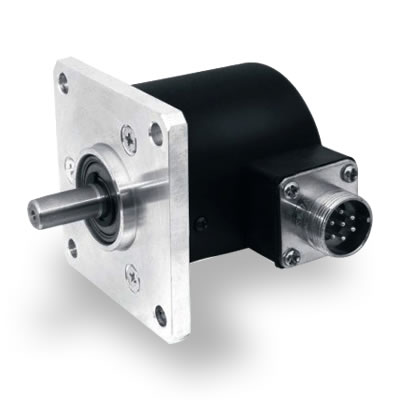
\includegraphics[width=0.4\textwidth]{thesis_figure/platformer_chapter/gdbmq}
	\caption{光电编码器}
	\label{fig:gdbmq}
\end{figure}
\subsection{采集卡}
数据采集系统是用来实时采样及保存发动机运行过程中各瞬态参数的。本试验采用NI公司出品的PCI 6250高速采集卡,其具备16路模拟信号输入,16
位转换精度,多通道采样频率1MHz,单通道模式下1.25MHz,最大采集幅值范围为±10V等强大功能。\par 研究爆震工况下的离子电流特性需要采集的参数
分为两大类:第一类是反映气缸内部燃烧状态及排放的信号,如缸内燃烧压力信号、离子电流信号及用于判断曲轴相位的A路和Z路信号等;二是发动机
ECU通过CAN总线发送出来的运行状态参数信号,如发动机转速、发动机负荷、爆震积分值、进气温度、进气压力、冷却水温度以及机油压力等等。该采
集卡能够满足以上两类需求。采集卡实物图如图\ref{fig:nicjk}所示,吊在空中是为了隔离干扰。
\begin{figure}[H]
	\centering
	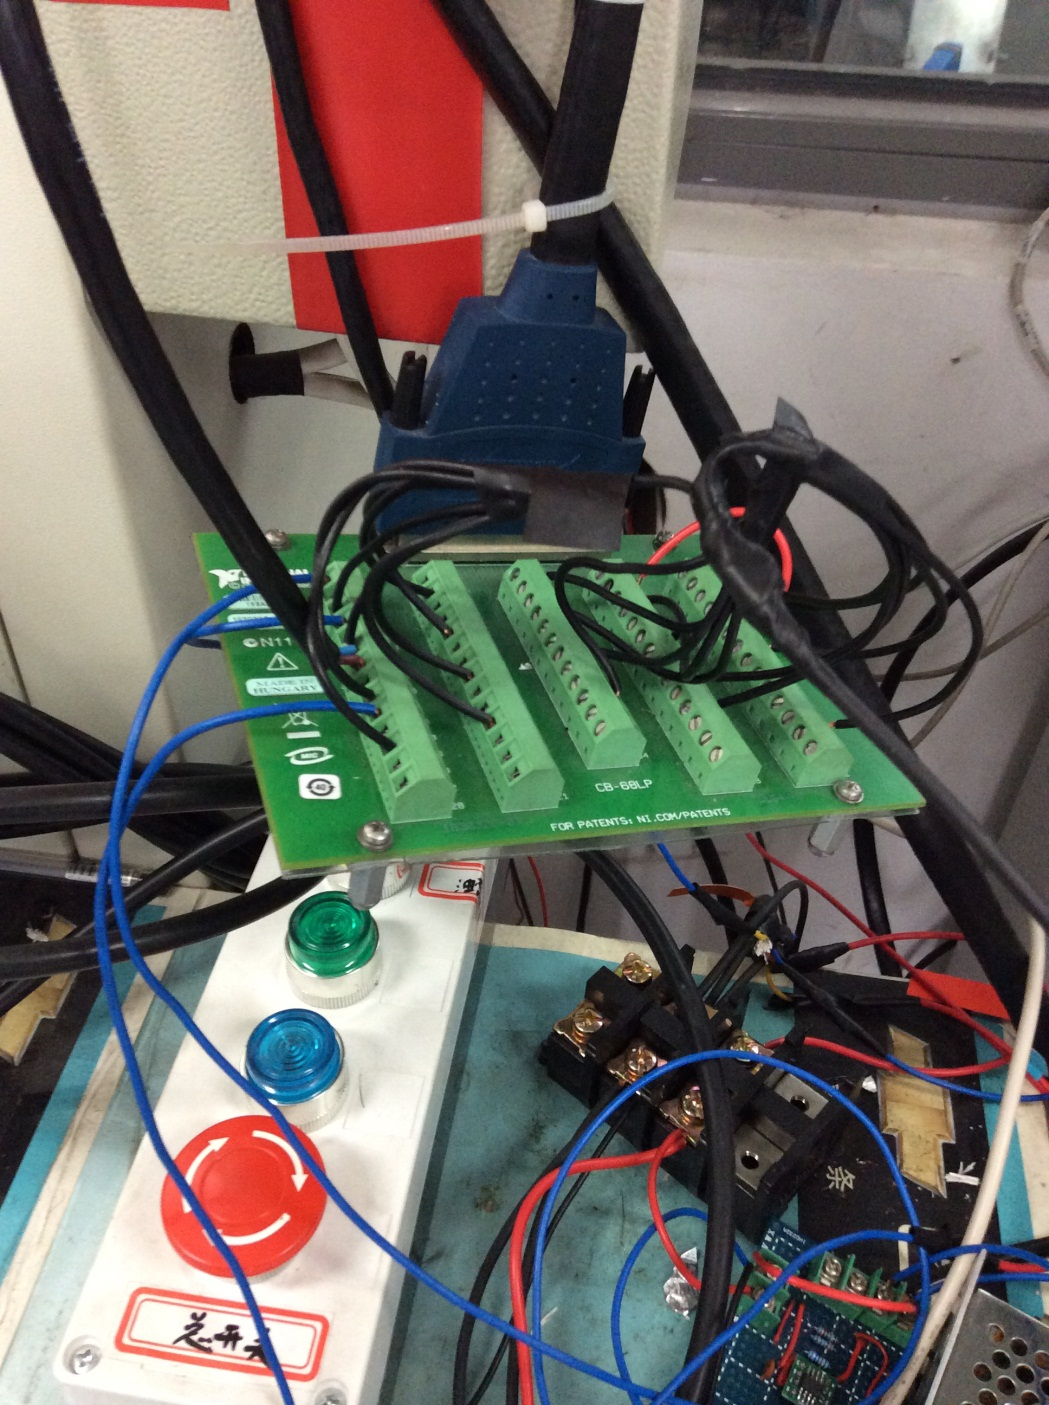
\includegraphics[width=0.4\textwidth]{thesis_figure/platformer_chapter/nicjk}
	\caption{NI公司提供的采集卡}
	\label{fig:nicjk}
\end{figure}
\subsection{采集程序}
采集程序是由Labview所编写,主要分为手动采集和触发采集两种类型,可通过记录模式进行切换。其中手动采集模式通过点击“开始”进行数据采
集,而触发采集可以设置触发条件,本文设置的是缸压值$>$阀值,采集程序会将超过该阀值的前后一段时间的数据采集下来,图\ref{fig:cjcxjm}是采集程序的界面。
\begin{figure}[!ht]
	\centering
	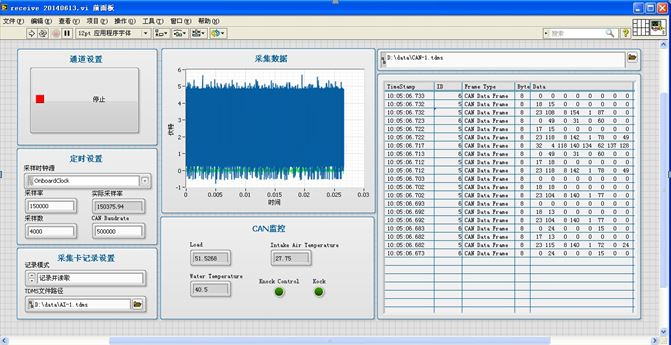
\includegraphics[width=0.9\textwidth]{thesis_figure/platformer_chapter/cjcxjm}
	\caption{采集程序界面}
	\label{fig:cjcxjm}
\end{figure}
\par 该采集程序主要由定时设置,采集卡记录设置,CAN监控,数据实时显示和通道开关几个部分组成。定时设置可以设置采样时钟、采样数、采样率等关键参数;采集卡记录设置
可以设置文件保存的路径,CAN监控可以实时监测采集过程是否有异常,同时也可以通过数据实时显示监控面板来查看数据采集过程是否有异常。





